\documentclass[twoside,twocolumn]{article}

\usepackage{blindtext} % Package to generate dummy text throughout this template 
\usepackage{graphicx}
\usepackage[sc]{mathpazo} % Use the Palatino font
\usepackage[T1]{fontenc} % Use 8-bit encoding that has 256 glyphs
\linespread{1.05} % Line spacing - Palatino needs more space between lines
\usepackage{microtype} % Slightly tweak font spacing for aesthetics

\usepackage[english]{babel} % Language hyphenation and typographical rules

\usepackage[hmarginratio=1:1,top=32mm,columnsep=20pt]{geometry} % Document margins
\usepackage[hang, small,labelfont=bf,up,textfont=it,up]{caption} % Custom captions under/above floats in tables or figures
\usepackage{booktabs} % Horizontal rules in tables
\usepackage{graphicx}
\usepackage{lettrine} % The lettrine is the first enlarged letter at the beginning of the text

\usepackage{enumitem} % Customized lists
\setlist[itemize]{noitemsep} % Make itemize lists more compact

\usepackage{abstract} % Allows abstract customization
\renewcommand{\abstractnamefont}{\normalfont\bfseries} % Set the "Abstract" text to bold
\renewcommand{\abstracttextfont}{\normalfont\small\itshape} % Set the abstract itself to small italic text

\usepackage{titlesec} % Allows customization of titles
\renewcommand\thesection{\Roman{section}} % Roman numerals for the sections
\renewcommand\thesubsection{\roman{subsection}} % roman numerals for subsections
\titleformat{\section}[block]{\large\scshape\centering}{\thesection.}{1em}{} % Change the look of the section titles
\titleformat{\subsection}[block]{\large}{\thesubsection.}{1em}{} % Change the look of the section titles

\usepackage{fancyhdr} % Headers and footers
\pagestyle{fancy} % All pages have headers and footers
\fancyhead{} % Blank out the default header
\fancyfoot{} % Blank out the default footer
\fancyhead[C]{Tecnologias OR-M $\bullet$ Agosto 2021 $\bullet$ } % Custom header text
\fancyfoot[RO,LE]{\thepage} % Custom footer text

\usepackage{titling} % Customizing the title section

\usepackage{hyperref} % For hyperlinks in the PDF

%----------------------------------------------------------------------------------------
%	TITLE SECTION
%----------------------------------------------------------------------------------------

\setlength{\droptitle}{-4\baselineskip} % Move the title up

\pretitle{\begin{center}\Huge\bfseries} % Article title formatting
\posttitle{\end{center}} % Article title closing formatting
\title{Tecnologias OR-M} % Article title
\author{Carlos Maldonado, Alfredo Huillca, Daniela Soto, Alexander Huallpa, Laura Condori}
\date{\today} % Leave empty to omit a date
\renewcommand{\maketitlehookd}{%

}

%----------------------------------------------------------------------------------------

\begin{document}

% Print the title
\maketitle

%----------------------------------------------------------------------------------------
%	ARTICLE CONTENTS
%----------------------------------------------------------------------------------------

\section{Resumen}

\lettrine[nindent=0em,lines=3]{L}a asignación de objetos relacionales es una técnica que le permite asignar cada una de las filas de nuestras
tablas en la base de datos de objetos, donde las columnas de la tabla corresponden a las propiedades de estos
objetos. La técnica, utilizada en la programación para convertir los tipos de datos con los que trabajan en un
lenguaje orientado a objetos, los tipos de datos con los que trabajan en un sistema de base de datos relacional
para la persistencia de datos en el objeto de mapeo-relacional. En el desarrollo de  una  aplicación  usando  el  paradigma  orientado  a  objetos,  los programadores  se enfrentan, entre otros desafíos, al problema de la persistencia de los datos, debido a las diferencias que existen  entre  el  modelo  relacional  y  el  modelo  orientado  a  objetos.Este  problema  la  mayoría  de  los casos  es  solucionado  con  la  ayuda  de  ciertas  herramientas  que  se  encargan  de  generar  de  manera automática el acceso a datos, abstrayendo al programador de este problema.



%------------------------------------------------

\section{Abstract}


The assignment of relational objects is a technique that would assign each of the rows of our
tables in the object database, where the columns of the table correspond to the properties of these
Objects. The technique, used in programming to convert the data types they work with into a
object-oriented language, the data types that you work with in a relational database system
for data persistence in the relational-mapping object. In developing an application using the object-oriented paradigm, programmers face, among other challenges, the problem of data persistence, due to the differences that exist between the relational model and the object-oriented model. Most of the cases are solved with the help of certain tools that are in charge of automatically generating access to data, abstracting the programmer from this problem.




%------------------------------------------------
\section{Introduccion}

ORM es el mapeo objeto-relacional (más conocido por su nombre en inglés, Object- Relational mapping), consiste
en una técnica de programación para convertir datos entre el lenguaje de programación
orientado a objetos utilizado y el sistema de base de datos relacional utilizado en el
desarrollo de aplicaciones. Esto posibilita el uso de las características propias de la
orientación a objetos (básicamente herencia y polimorfismo). Entre estos paquetes comerciales tenemos
una lista alfabética de los principales motores de mapeo objeto relacional, tales como:
ColdFusion, Common Lisp, Java, JavaScript, .NET, Perl, PHP, Python, Ruby, Smalltalk, C++. El problema que surge, porque hoy en
día prácticamente todas las aplicaciones están diseñadas para usar la Programación
Orientación a Objetos (POO), mientras que las bases de datos más extendidas son del
tipo relacional y estas solo permiten guardar tipos de datos primitivos (enteros, cadenas
de texto) por lo que no se puede guardar de El problema que surge, porque hoy en
día prácticamente todas las aplicaciones están diseñadas para usar la Programación
Orientación a Objetos (POO), mientras que las bases de datos más extendidas son del
tipo relacional y estas solo permiten guardar tipos de datos primitivos (enteros, cadenas de texto) por lo que no se puede guardar de forma directa los objetos de la aplicación en las tablas, sino que estos se deben de convertir antes en registros, que por lo general afectan a varias tablas. En el momento de volver a recuperar los datos, hay que hacer el proceso contrario, se deben convertir los registros en objetos.
 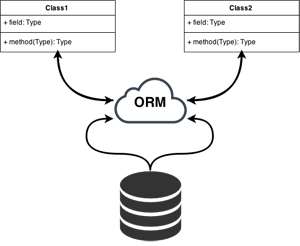
\includegraphics[width=7cm, height=7cm]{imagenes/ORM.png}

\section{Desarrollo}

\subsection{¿Qué es un ORM?}

Hoy hablamos del Mapeo Objeto Relacional o como se conocen comunmente, ORM, Algunos de vosotros ya 
sabréis que son pero, para aquellos que
no los conozcan, un ORM te permite
convertir los datos de tus objectos en un
formato correcto para poder guardar la
información en una base de datos (mapeo)
creándose una base de datos virtual
donde los datos que se encuentran en
nuestra aplicación, quedan vinculados a
la base de datos (persistencia). Si alguna vez has programado alguna aplicación que se conecta a una base de
datos, que estes utilizando en ese momento pudiendo cambiar de motor de base de datos segun tus necesidades.
Veamos un ejemplo. Supongamos que tenemos una tabla de clientes. En nuetra aplicacion queremos hacer las funciones basicas
sobre base de datos CRUD, Crear Obtener,Actualizar y Borrar, Cada operacion corresponde con una sentencia SQL. 
\begin{itemize}
	\item Crear: INSERT
	\item Obtener: SELECT
	\item Actualizar: UPDATE
	\item Borrar: DELETE
\end{itemize}



\subsection{Herramientas ORM}

En el mercado podemos encontrar divesas herramientas tanto de pago como de uso libre. Algunos programadores, 
prefieren invertir tiempo en desarrollar su propia herramienta ORM usando patrones de diseño bien conocidos como 
son el Repository o el Active Record.

El patron Repository se soporta sobre la definicion de un repositorio para separar la logica que recupera los datos de 
la base de datos de la logica de negocio basada en objetos. Este repositorio hace de puente entre los datos y las operaciones basadas
en objetos, eliminando dependencias tecnologicas y facilitando el acceso a datos de cualquier tipo.
Por otro lado, esta el patron Active Record. Es un patron en el cual, el objeto contiene los datos que representan a un registro de 
nuestra tabla o viste relacional, ademas de encapsular la logica necesaria para acceder a la base de datos. De esta forma el acceso a datosse presenta de manera uniforme a travez
de la aplicacion(logica de negocio + acceso a datos en una misma clase).

Las herramientas ORM que hay en el mercado son diversas. Algunas estan ligadas al lenguaje de programacion orientado a objetos especifico.
Algunos ejemplos especificos serian: 

\begin{itemize}
\item Para Java: Hibernate, iBatis, Ebean, Torque.
\item Para .Net: nHibernate, Entity Framework, DataObjects.Net
\item Para PHP: Doctrine, Propel, Torpor
\item Para Pytho: SQLObject, Django, Tryton.


\end{itemize}

\subsection{Ventajas e inconvenientes de las Herramientas ORM}

Las herramientas ORM ofrecen ventajas para el programador como son:
 \begin{itemize}
	 \item Rapidez en el desarrollo
	 \item Abstraccion de la base de datos utilizada
	 \item Seguridad de la capa de acceso
	 \item Facilidad para el mantenimiento del codigo
	 \item lenguaje propio para la realizacion de consultas
	\item El aprendizaje del lenguaje de la herramienta ORM puede resultar ser complejo ya que, para poder sacar el máximo partido            a la herramienta, es necesario conocer en profundidad cómo funciona la misma.
          \item En entornos de gran carga, este tipo de solución penaliza el rendimiento debido a los procesos de transformación de las  consultas que se hagan hacia la base de datos.
 \end{itemize}
 \subsection{Herramienta Entity Framework}
 Entity Framework es el ORM de Microsoft, con versiones tanto para la plataforma .NET "tradicional"
 como para .NET Core. 
 Como vimos en el articulo del enlace anterior, en el que se expliocaba con detalle que es un ORM, este tipo de software
 puede funcionar de varias maneras diferentes a la hora de "mapear" las clases de nuestro programa orientado a objetos y las tablas en la 
 base de datos 
 Entity Framework no es una excepcion, y nos ofrece diversas maneras de trabajar con los datos desde nuestros porgramas. 
 Cadda una tieneun enfoque diferente y es interesante para ciertos casos concretos, ademas de tener sus beneficios y problemas.
 Es importante tener en cuenta que las capacidades de Entity Framework en .NET "tradicional" y en .NET core son copletamente 
 diferentes.
Asi los tres modos de trabajo descritos a continuacion estan completamente soportados en EF6, pero EF Core solamente soporta "Code First" en .NET
Core ni esta ni se le espera.
 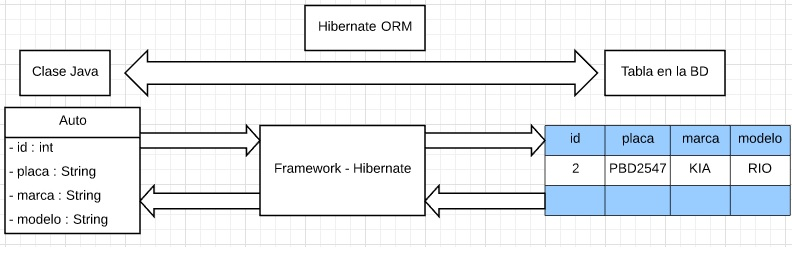
\includegraphics[width=7cm, height=7cm]{imagenes/hibernate.jpg}
\section{Conclusiones}
El uso de un ORM es una alternativa sumamente efectiva a la hora de trasladar el modelo conceptual(orientado a objetos)
al esquema relacional nativo de la bas bases de datos SQL. Evita la inclusion de sentencias SQL embebidas en el codigo de la aplicacion, lo que a su vez facilita la migracion
hacia otro sistemas gestor de bases de datos, Incorpora una capa de abstraccion. Al ser realizado, en esta capa, de manera automatica la conversion de 
instrucciones orientadas a objetos, a sentencias SQL, minimiza la ocurrencia de errores humanos.

De cualquier modo, utilizar un ORM no debe ser considerado una panacea, sino que debe usarse a discrecion; teniendo en cuenta las 
particularidades de cada problema a modela. En determinados casos no es recomendable el uso de un ORM,
sobre todo cuando se imponen tiempos de respuesta minimos o se requiere una menor sobrecarga. En estos casos lo mas conveniente es el uso de un 
microORM; evitando siempre que sea posible las inyecciones de SQL Inline.
\section{Recomendaciones}
 \begin{itemize}
\item El uso de mapeo objeto relacional(ORM), es esencial en los tiempos actuales, debido a que la mayoria de lenguajes de programacion poseen un paradigma orientado a objetos, pues simplifica grandemente el
desarrollo de la capa de persistencia, tratándose de una idea madura y
que cada día gana más popularidad. 

\item Los ORM son diferentes, por lo debe verificar el que mas se adecue al desarrollo del proyecto y los requerimientos del mismo.

\item En la actualidad existen varias herramientas ORM, tanto de codigo abierto y comerciales. Por lo que es recomendable elegir solo una.
 \end{itemize}
%----------------------------------------------------------------------------------------
%	REFERENCE LIST
%----------------------------------------------------------------------------------------

\begin{thebibliography}{XXX0000}
	\bibitem - MSDN, The Microsoft Developer Network. Local Help, Visual Studio 2008. Disponible en: http://msdn.microsoft.com/en-us/
	\bibitem - Introducción a Object-Relational Mapping (ORM). Iván Guardado. Mayo 2010. Disponible en: http://web.ontuts.com/tutoriales/introduccion-a-object-relational-mapping-orm/
	\bibitem - Introducción al Desarrollo de Aplicaciones con Bases de Datos. Alarcos. Departamento de Tecnologías y Sistemas de Información de la Universidad de Castilla. Enero 2007. Disponible en: http://alarcos.esi.uclm.es/doc/aplicabbdd/Documentos/teoria/introducci%C3%B3n%20al%20desarrollo%20aplicaciones%20con%20bases%20de%20datos.pdf
	\bibitem - Impedance Mismatch. Kazimierz Subieta. Enero 2008. Disponible en: http://www.sbql.pl/Topics/ImpedanceMismatch.html
	\bibitem - Patrones de Acceso a Datos: Active Record. Grimpi IT. Febrero 2009. Disponible en: http://grimpidev.wordpress.com/2008/11/22/patrones-de-acceso-a-datos-active-record/
	\bibitem - Active Record. Néstor Salceda. Septiembre 2009. Disponible en: http://es.debugmodeon.com/articulo/active-record
	\bibitem - Getting Started with SubSonic. Scott Kuhl. Noviembre 2006. Disponible en:http://geekswithblogs.net/scottkuhl/archive/2006/11/16/97298.aspx
	\bibitem - Juan Maria Hernandez (2016) Los Patrones de Diseño Hoy: Patrones de Comportamiento. Recuperado 7 de Abril 2021, de https://blog.koalite.com/2016/12/los-patrones-de-diseno-hoy-patrones-de-comportamiento/
	\bibitem - Autocompletado del código SQL, herramientas de subversión, desarrollo ágil, y más. James Avery. Febrero 2008. Disponible en: http://msdn.microsoft.com/es-es/magazine/cc164246.aspx
	\end{thebibliography}

%----------------------------------------------------------------------------------------

\end{document}